\documentclass{beamer}[10pt]
\usetheme{Luebeck}
\usecolortheme{beaver}
\usepackage[utf8]{inputenc}
\usepackage{amsmath,amsfonts,amssymb,amsthm}
\usepackage{bbm}
\usepackage{color}
\usepackage{mathtools}

\setbeamercolor{block title}{bg=gray!50,fg=black}
\setbeamercolor{itemize item}{fg=red} 

\title{Alternating Homology}
\author{Josef Dean }
\date{May 2016}

\usepackage{natbib}
\usepackage{graphicx}
\usepackage[all]{xy}



\DeclareMathOperator{\Ima}{Im}
\DeclareMathOperator{\Ker}{Ker}
\DeclareMathOperator{\Tor}{Tor}
\DeclareMathOperator{\Rank}{Rank}
\DeclareMathOperator{\co}{\!\colon\!}
\DeclareMathOperator{\Alt}{Alt}
\DeclareMathOperator{\sgn}{sgn}
\DeclareMathOperator{\supp}{supp}
\DeclareMathOperator{\diam}{diam}
\DeclareMathOperator{\coloneqq}{\vcentcolon=}

\newcounter{thm}

\theoremstyle{definition}
\newtheorem{defn}[thm]{Definition}



\begin{document}

\begin{frame}
\titlepage
\end{frame}

\section{Motivation}

\begin{frame}
\frametitle{Motivation}
$$f\co X\longrightarrow Y$$
\vspace{4mm}
{\small $$D^k(f)=\text{closure}\{(x_1,\dots,x_k)\in X^k\,|\,f(x_1)=...=f(x_k),\, x_i\neq x_j\,\text{if}\,i\neq j\}$$}
\vspace{4mm}
$$\pi_k:D^k(f)\longrightarrow D^{k-1}(f)$$
\vspace{3mm}
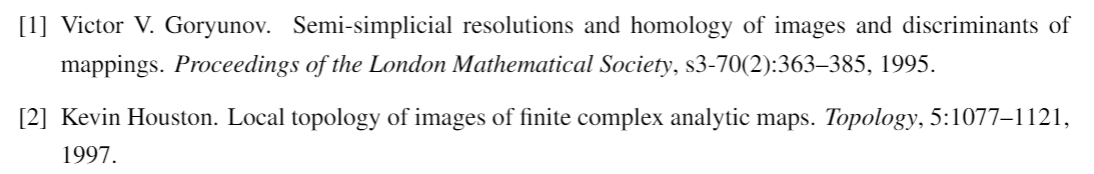
\includegraphics[scale=0.38]{MotivationSources.PNG}
\end{frame}

\begin{frame}[t]
\frametitle{Image Computing Spectral Sequence}
\begin{displaymath}
\xymatrix@R=0.5cm@C=0.55cm{
& \vdots \ar[d] & \vdots \ar[d] & \vdots \ar[d] & \\
\dots \ar[r]^{\partial\quad\quad} & C_{n\!+\!1}^{alt}(D^{k+1}(f)) \ar[r]^\partial \ar[d]^{\pi_{k+1\#}}  & C_{n}^{alt}(D^{k+1}(f)) \ar[r]^{\partial\quad} \ar[d]^{\pi_{k+1\#}}  & C_{n\!-\!1}^{alt}(D^{k+1}(f)) \ar[r]^{\quad\quad\partial} \ar[d]^{\pi_{k+1\#}}  & \dots \\
\dots \ar[r]^{\partial\quad\quad} & C_{n\!+\!1}^{alt}(D^{k}(f)) \ar[r]^\partial \ar[d]^{\pi_{k\#}}  & C_{n}^{alt}(D^{k}(f)) \ar[r]^{\partial\quad} \ar[d]^{\pi_{k\#}}  & C_{n\!-\!1}^{alt}(D^{k}(f)) \ar[r]^{\quad\quad\partial} \ar[d]^{\pi_{k\#}}  & \dots \\
\dots \ar[r]^{\partial\quad\quad} & C_{n\!+\!1}^{alt}(D^{k-1}(f)) \ar[r]^\partial \ar[d]  & C_{n}^{alt}(D^{k-1}(f)) \ar[r]^{\partial\quad} \ar[d] & C_{n\!-\!1}^{alt}(D^{k-1}(f)) \ar[r]^{\quad\quad\partial} \ar[d] & \dots \\
& \vdots & \vdots & \vdots &
}
\end{displaymath}
\end{frame}

\section{Definitions}

\begin{frame}
\frametitle{$S_k$-space}
\centering
A topological space $X$ acted on by symmetric group $S_k$.

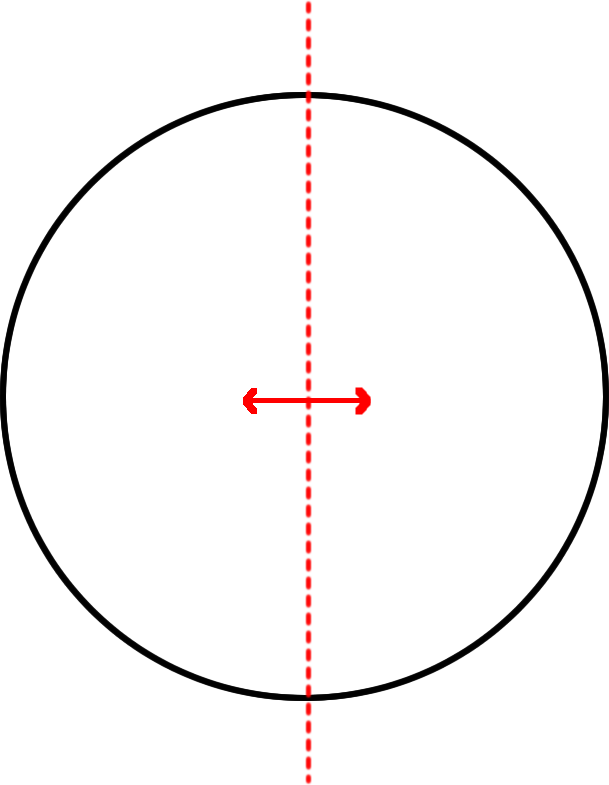
\includegraphics[scale=0.15]{S2Space.png}

$k=2$
\end{frame}

\begin{frame}
\frametitle{Alternating Singular Homology}
\centering
$$C^{alt}_n(X)=\{c\in C_n(X) \,| \,\sigma_\#(c)\!=\!\sgn(\sigma)c\quad\forall\sigma\in S_k\}$$
$$H_n^{alt}(X)=\frac{\Ker\partial}{\Ima\partial}$$
\vspace{3mm}
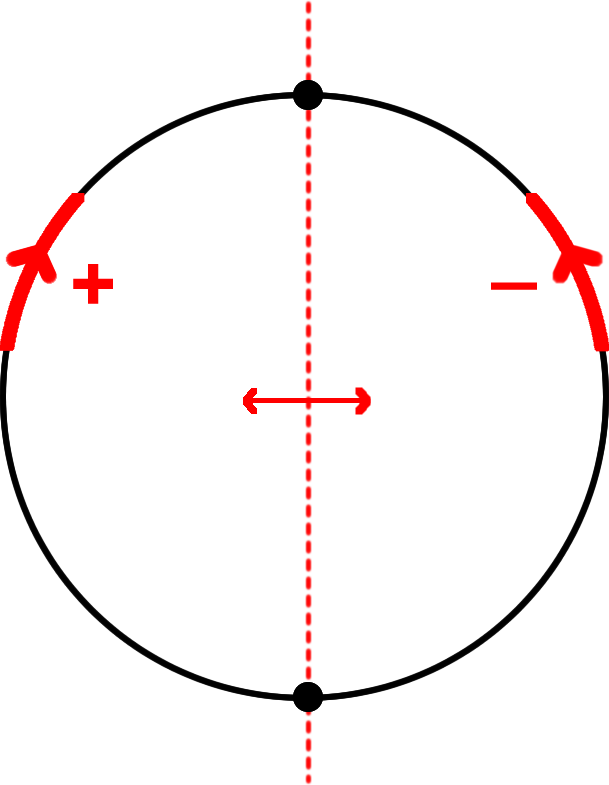
\includegraphics[scale=0.15]{Alternating1Chain.png}
\end{frame}


\section{Differences with (ordinary) homology}

\begin{frame}
\frametitle{Trivial space}
\centering
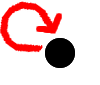
\includegraphics[scale=0.2]{trivialSpace.png}
$$\forall \sigma\in S_k\quad\sigma x=x$$
$$k>1\,\implies\,C_n^{alt}(\{x\})=0\quad \forall n$$
\end{frame}

\begin{frame}
\frametitle{Connected components}
\begin{columns}[T] % align columns
\begin{column}{.47\textwidth}
\centering
Homology
\small$$H_n(\{x_0,x_1\})\cong H_n(\{x_0\})\oplus H_n(\{x_1\})$$
\vspace{1cm}
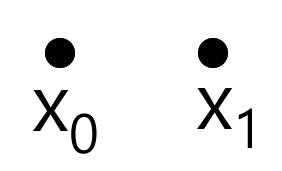
\includegraphics[scale=0.15]{twopoints.png}
\end{column}%
\begin{column}{.03\textwidth}
\centering
\rule[-1mm]{0.5mm}{6cm}%
\end{column}%
\begin{column}{.47\textwidth}
\centering
Alternating Homology
$$H^{alt}_0(\{x_0,x_1\})\cong \mathbb{Z}$$
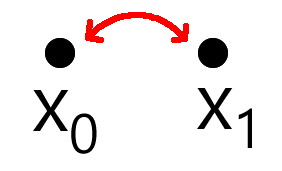
\includegraphics[scale=0.15]{twopointsPermuted.png}
$$H^{alt}_0(\{x_0\})\oplus H^{alt}_0(\{x_1\})\cong0\oplus0$$
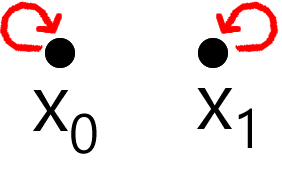
\includegraphics[scale=0.15]{twopointsSplit.png}
\end{column}%
\end{columns}
\end{frame}


\begin{frame}
\frametitle{Reduced Homology}
$$...\longrightarrow C_2(X)\overset\partial\longrightarrow C_1(X) \overset\partial\longrightarrow C_0(X)\overset\varepsilon\longrightarrow \mathbb{Z}\longrightarrow 0$$
$$\varepsilon(\Sigma\alpha_i\sigma_i)=\Sigma\alpha_i $$
\vspace{12mm}
$$c=\Sigma\alpha_ic_i\in C^{alt}_n(X),\quad\sigma_\#(\Sigma\alpha_ic_i)=\Sigma(-\alpha_i)c_i$$
\end{frame}



\section{Results}

\begin{frame}
\frametitle{$S_k$-homotopy invariance}
\centering
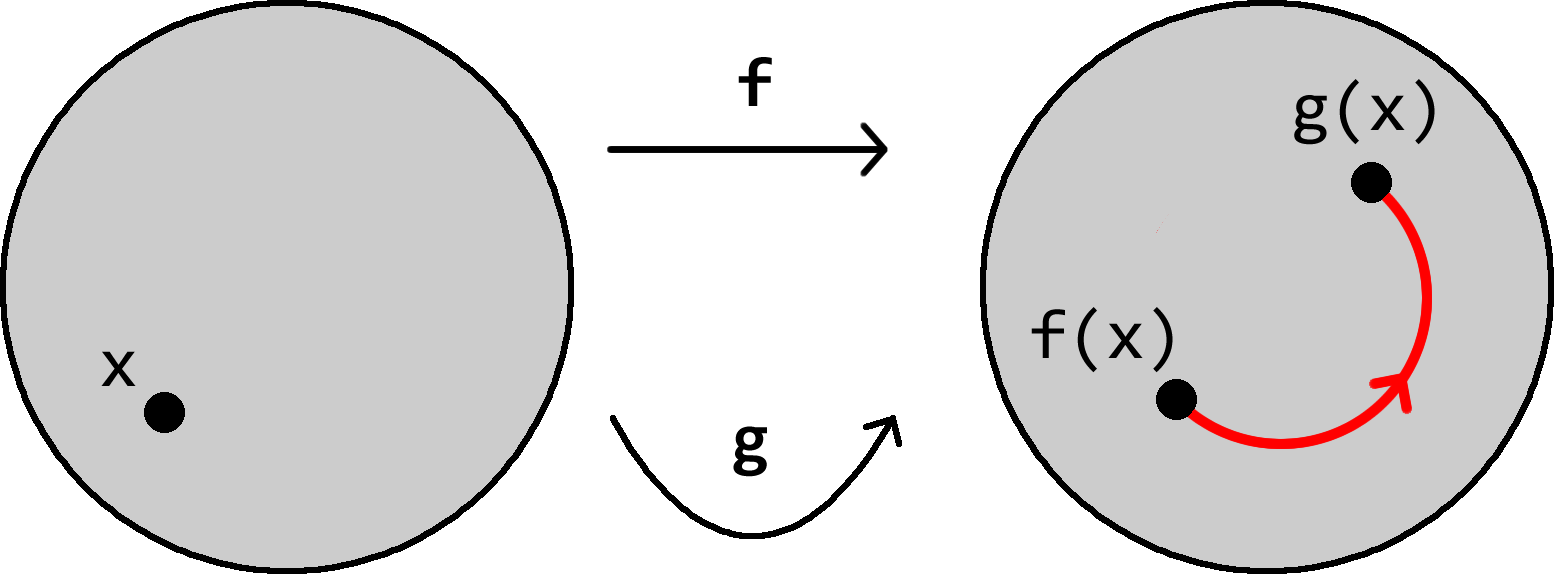
\includegraphics[scale=0.15]{prism.png}
\end{frame}

\begin{frame}
\frametitle{$S_k$-homotopy invariance}
\centering
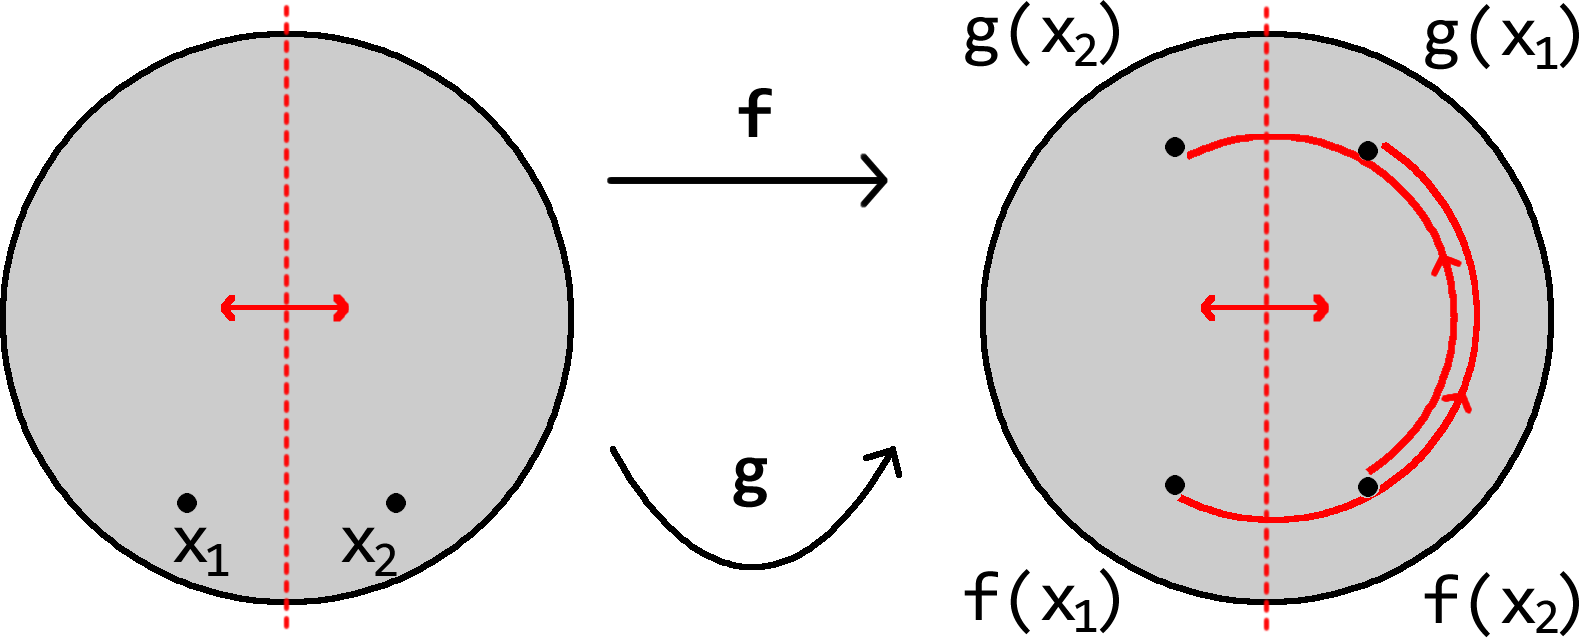
\includegraphics[scale=0.15]{nonequivariantPrism.png}
\end{frame}

\begin{frame}
\frametitle{$S_k$-homotopy invariance}
\begin{block}{Definition}
For $f,g\colon X\to Y$ an $S_k$-homotopy $F\colon X\times I\longrightarrow Y$ is a homotopy from $f$ to $g$ that is equivariant in the first argument.\\
$F(\sigma x,t)=\sigma F(x,t)\quad \forall t\in I,\,\forall\sigma\in S_k$.
\end{block}
\centering
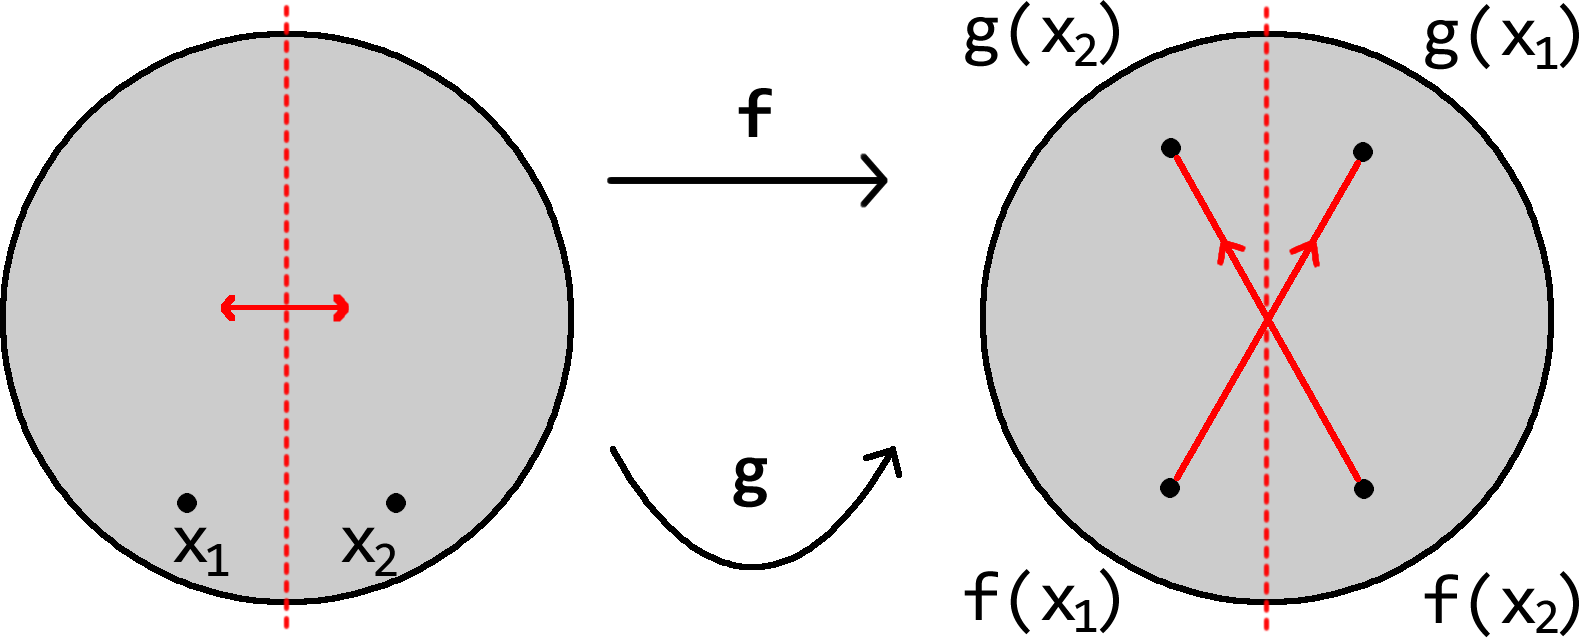
\includegraphics[scale=0.15]{equivariantPrism.png}
\end{frame}





\begin{frame}
\frametitle{Excision}
\centering
\begin{block}{Relative Alternating Chain Groups}
For $A\subset X$ an $S_k$-subspace, $\quad C^{alt}_n(X,A)\coloneqq \frac{C_n^{alt}(X)}{C_n^{alt}(A)}$
\end{block}
\begin{block}{Theorem}
For $S_k$-space $X$ and $S_k$-subspaces $Z\subset A\subset X$ where $\overline{Z}\subset\overset{\,\circ}A$, the inclusion $(X\setminus Z,A\setminus Z)\hookrightarrow(X,A)$ induces isomorphisms $H^{alt}_n(X\setminus Z,A\setminus Z)\cong H^{alt}_n(X,A)$.
\end{block}
\begin{block}{Theorem}
For $S_k$-subspaces $A,B\subset X$, where $\overset{\,\circ}A\cup\overset{\,\circ}B=X$, the inclusion $(B,B\cap A)\hookrightarrow(X,A)$ induces isomorphisms $H^{alt}_n(B,B\cap A)\cong H^{alt}_n(X,A)$.
\end{block}
\end{frame}

\begin{frame}
\frametitle{Excision}
\centering
$$\mathfrak{i}\vcentcolon C^{alt}_n(A+B)\hookrightarrow C^{alt}_n(X) \quad\quad \rho\vcentcolon C^{alt}_n(X)\rightarrow C^{alt}_n(A+B)$$
$$\partial D+D\partial=\mathbbm{1}-\mathfrak{i}\rho\,\text{ and }\,\rho\mathfrak{i}=\mathbbm{1}$$
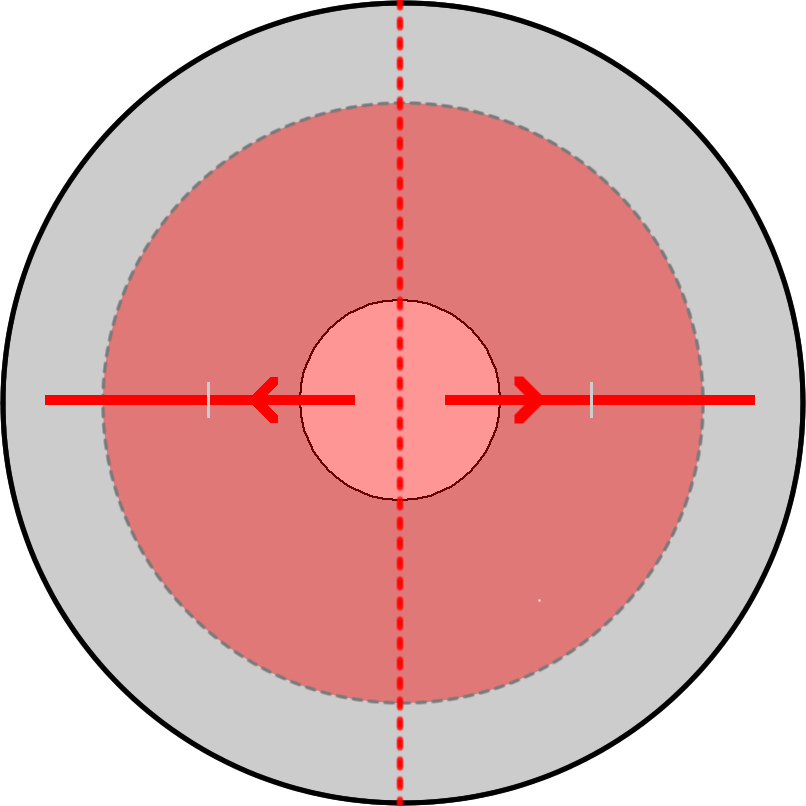
\includegraphics[scale=0.15]{subdivision.png}
\end{frame}

\begin{frame}
\frametitle{Excision}
\centering
$$H^{alt}_n(\frac{C^{alt}_n(X)}{C^{alt}_n(A)})\overset{\mathfrak{i}}\cong H^{alt}_n(\frac{C^{alt}_n(A+B)}{C^{alt}_n(A)})\cong H^{alt}_n(\frac{C^{alt}_n(B)}{C^{alt}_n(A\cap B)})$$
$$H^{alt}_n(X,A)\cong H^{alt}_n(B,B\cap A)$$
\end{frame}



\begin{frame}
\frametitle{Good $S_k$-pair}
\centering
\begin{block}{Definition}
For $A\subset X$ a non-empty closed $S_k$-subspace, $(X,A)$ is a Good $S_k$-pair if $A$ is an equivariant deformation retract of some neighbourhood $V$, another $S_k$-subspace of $X$.
\end{block}
$H^{alt}_n(X,A)\cong H^{alt}_n(X/A)$
\end{frame}



\section{Computation}


\begin{frame}
\frametitle{Simplicial Alternating Homology}
\centering
If the action of $S_k$-space $X$ induces an action of $S_k$ on simplicial chain groups $\triangle_n(X)$ for some $\Delta$-complex,
$$\triangle_{n}^{alt}(X) \coloneqq \{ c \in \triangle_n(X) \mid \sigma_\#(c) = \sgn(\sigma)c \quad \forall \,\sigma \in S_k\}$$

\begin{columns}[T] % align columns
\begin{column}{.4\textwidth}
\centering
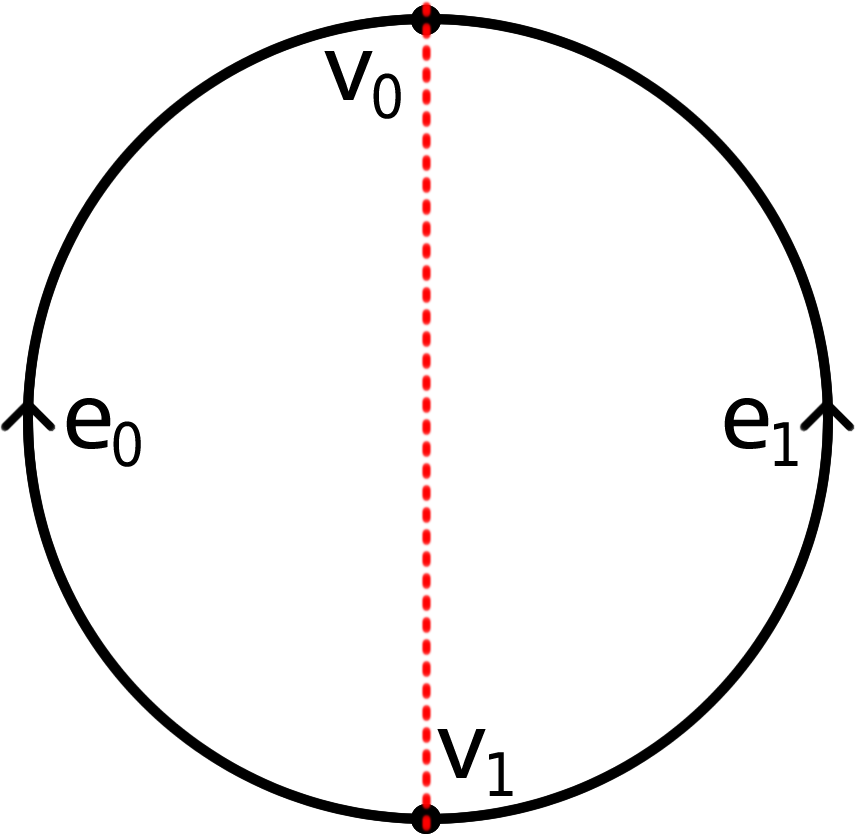
\includegraphics[scale=0.15]{simplicialS1.png}
\end{column}%
\begin{column}{.58\textwidth}
\centering
\vspace{3mm}
$$H^{alt}_{n,\triangle}(X)=\begin{cases} \mathbb{Z} & n=1 \\ 0 & n\neq1\end{cases}$$
\vspace{3mm}
$$H^{alt}_{n,\triangle}(X)\cong H^{alt}_n(X)$$
\end{column}%
\end{columns}
\end{frame}


\begin{frame}
\frametitle{Computation}
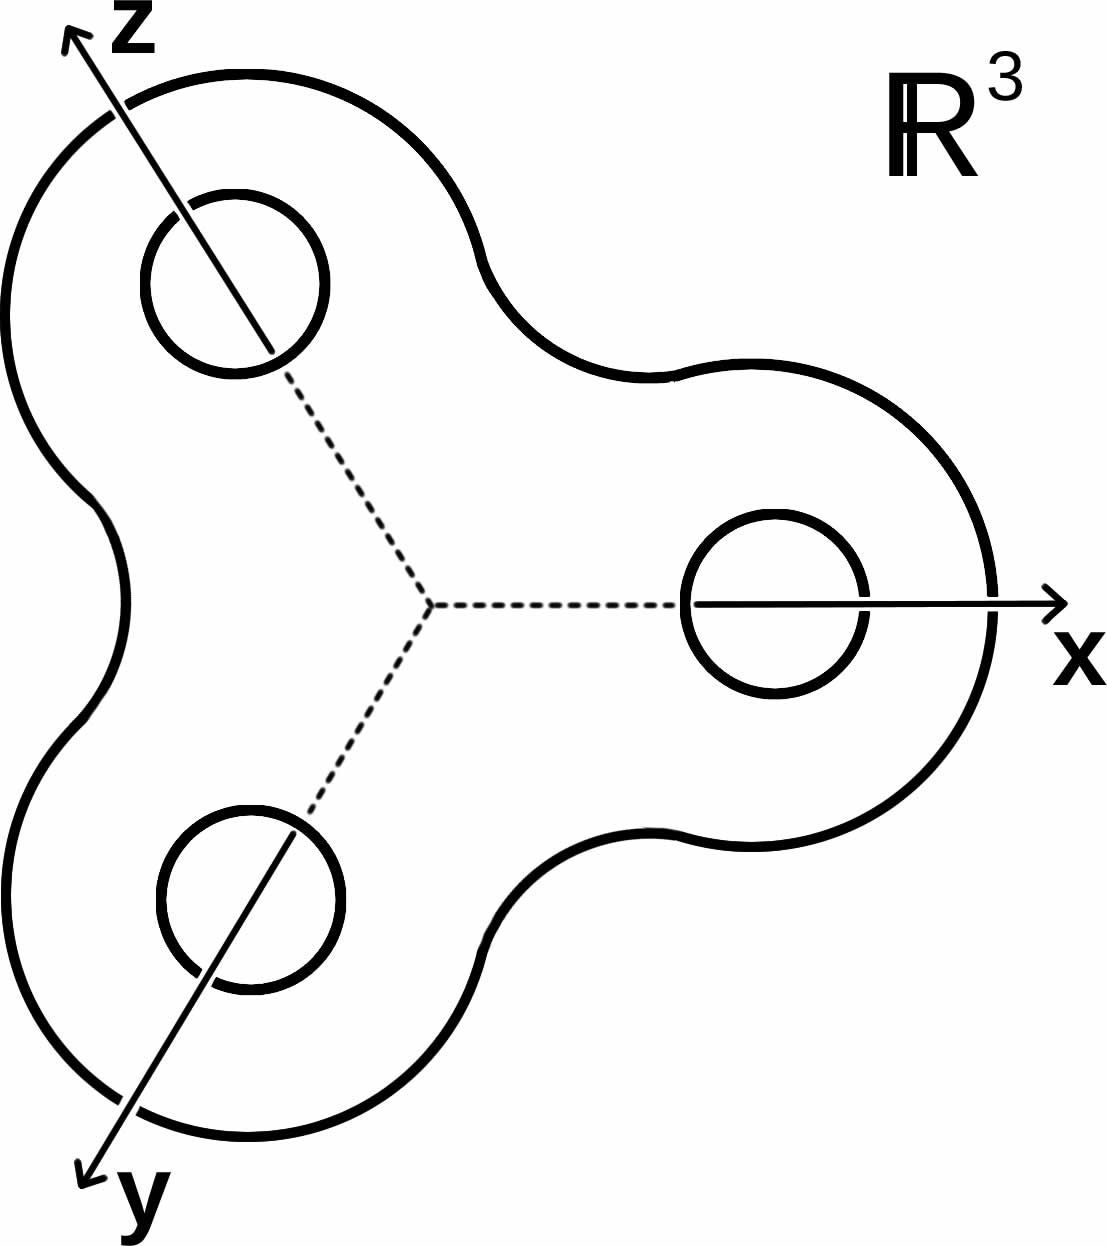
\includegraphics[scale=0.12]{Genus3ActionCrossSection.jpg}
\hfill
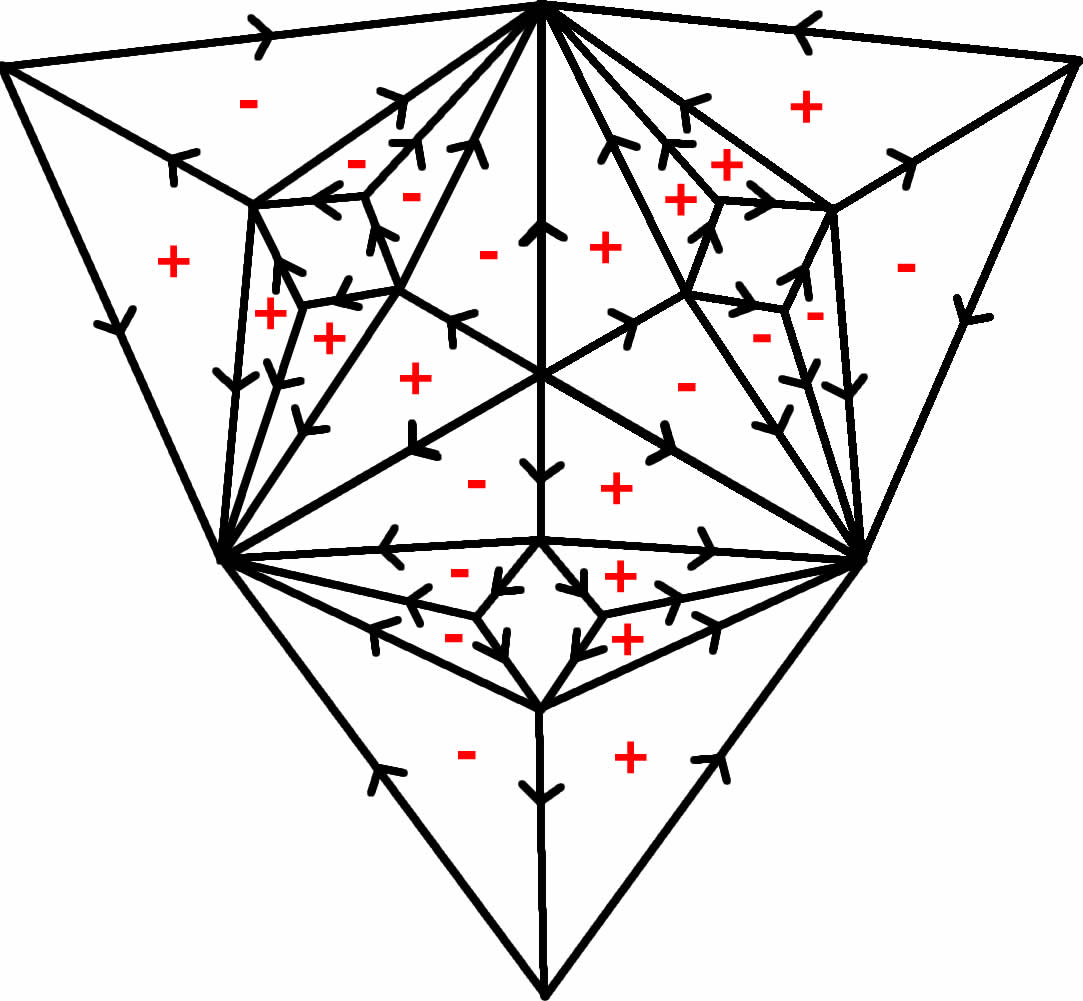
\includegraphics[scale=0.12]{Genus3ActionDeltaComplex.jpg}
\end{frame}

\begin{frame}
\frametitle{Computation}
\centering
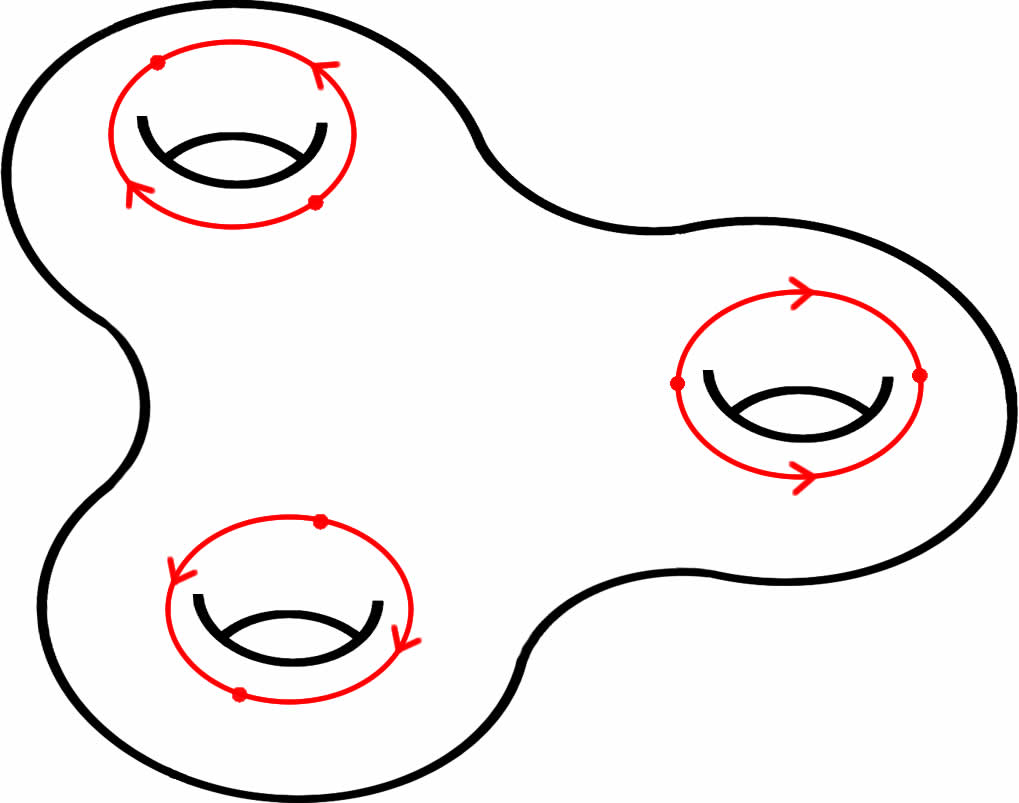
\includegraphics[scale=0.15]{Genus3AltHom1Generator.jpg}
\end{frame}



\begin{frame}
\frametitle{Links to other theory}
\begin{itemize}
\item Alternating Homology with Rational Coefficients \\
   $\quad\quad \text{Alt}H_n(X;\mathbb{Q})\cong H^{alt}_n(X;\mathbb{Q})\cong H^{alt}_n(X)\otimes_\mathbb{Z}\mathbb{Q}$
   \vspace{3mm}
\item Alternating Homology as Homology with Local Coefficients
\end{itemize}
\end{frame}


\end{document}
